\begin{tcolorbox}[
  colback=cyan,
  colframe=cyan,
  coltext=white, 
  halign=center,
  sharp corners,
]
ПРОГУЛКИ С ФИЗИКОЙ
\end{tcolorbox}

\noindent
\begin{minipage}[t]{0.25\textwidth}
\vspace{0pt}
сматривать колебания каждого атома независимыми. При одинаковом устройстве внешних оболочек атомов, которым определяется вид зависимости энергии взаимодействия соседних атомов друг с другом от расстояния 
\end{minipage}
\begin{minipage}[t]{0.75\textwidth}
\vspace{0pt}
\noindent
\makebox[\linewidth][r]{
  \setlength{\tabcolsep}{3pt}
  \begin{tabular}{|c|c|c|c|c|c|c|c|c|c|c|c|c|}
  \hline
  Hg & Se & K & Pb & Bi & Te & Na & Au & S & Sn & U & Sb & \makecell{Sn\\серое} \\ \hline
  75 & 89 & 90 & 95 & 117 & 153 & 160 & 165 & 180 & 190 & 200 & 204 & 212 \\ \hline\hline
  Ag & Pt & V & Pd & Ti & Cd & Zn & Cu & Li & W & Ge & \makecell{C\\графит} & Al \\ \hline
  225 & 233 & 273 & 275 & 278 & 300 & 305 & 343 & 354 & 367 & 370 & 391 & 398 \\ \hline\hline
  Cr & Mg & Ir & Mo & Co & Mn & Ni & Fe & Os & Ru & Si & Be & \makecell{C\\алмаз} \\ \hline
  402 & 405 & 420 & 425 & 445 & 450 & 465 & 467 & 500 & 600 & 658 & 1160 & 1860 \\ \hline
  \end{tabular}
}
\end{minipage}

\begin{multicols}{2}
\noindent
между их центрами, частота колебаний тем меньше, чем больше масса атомов. Если температура твердого вещества такова, что выполняется неравенство

\[
kT > \hbar\omega_{\text{max}} , \eqno{(8)}
\]

\noindent
то в этом диапазоне температур закон Дюлонга и Пти для этого вещества справедлив. Соответствующая граничная температура называется температурой Дебая:

\[
T_{\text{Дебая}} = \frac{\hbar\omega_{\text{max}}}{k} .
\]

\noindent
Здесь приведена таблица значений температуры Дебая (в кельвинах) для простых веществ). Тенденцию уменьшения температуры Дебая с ростом массы атомов веществ

\columnbreak

\noindent
с похожими химическими свойствами можно увидеть на примере таких групп веществ: а) медь, серебро, золото; б) алмаз, кремний, германий, олово, свинец; в) литий, натрий, калий. Для бериллия и алмаза, например, температуры Дебая равны примерно \(10^3\)~К и \(2 \cdot 10^3\)~К. Поэтому для этих веществ закон Дюлонга и Пти при нормальных (комнатных) температурах не выполняется.

\medskip
* * *
\medskip

Как вы заметили, во все формулы, ограничивающие «классику» в области молекулярно-кинетической теории, входит основная квантовая величина \(\hbar\). В формуле (5), правда, она «спрятана» в \(\Delta U\).

\end{multicols}

\begin{tcolorbox}[
  colback=cyan,
  colframe=cyan,
  coltext=white, 
  halign=center,
  sharp corners,
  width=0.7\textwidth,
  height=0.1\textwidth,
  center,
]
\vspace{10pt}
ПРОГУЛКИ С ФИЗИКОЙ
\end{tcolorbox}

\begin{multicols}{2}
{\centering
\large\textbf{Узоры под скамейкой}\\[5pt]
\small\textit{(Начало см. на 4-й странице обложки)}
\par}
\vspace{-15pt}

Посмотрите на фотографии, приведенные здесь и на обложке. Оказывается, узоры под скамейкой нарисованы… мхом. Эти фотографии заставляют вспомнить и об известной примете — мох растет на северной стороне дерева, и о мегалитических сооружениях (например, знаменитом Ньюгрейндже в Ирландии) — сюда солнечный свет попадает раз в году. Подробную информацию и о том и о другом, а также очень красивые картинки можно найти по ключевым словам в интернете.

Решетчатая структура сидений скамеек вместе с их расположением на лесной поляне (где окружающие деревья ограничивают распространение прямого солнечного света) и характером суточного движения солнца по небосводу обеспечивают неравномерное проникновение света под скамейки в течение суток. А пространственное распределение солнечной освещенности визуализируется мхом.

\columnbreak

\begin{center}
    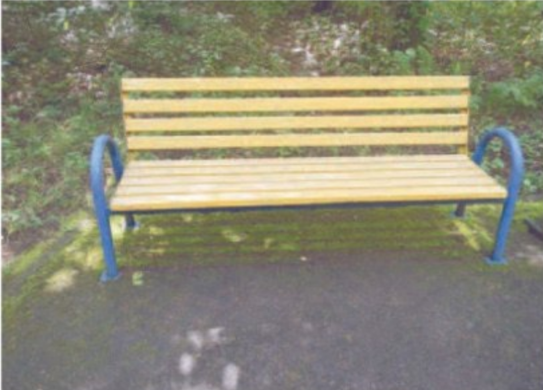
\includegraphics[width=0.5\textwidth]{image.png}
\end{center}

Правда, на фотографиях можно заметить, что мох растет скорее на освещенных, нежели на теневых участках земли. Вероятно, в отличие от роста мха на деревьях, в данном случае из двух факторов — доступности влаги и доступности освещения — освещение оказывается доминирующим. (Впрочем, здесь явно сказывается еще и третий фактор — вытаптывание.)

\begin{flushright}
\textit{В. Птушенко}
\end{flushright}

\end{multicols}
